\section{Обзор архитектуры RISC-V}
\label{riscv} \index{riscv}

\subsection {Общая информация}
\label{riscv:general}

RISC-V -- это архитектура команд (ISA), основанная на принципах сокращённого
набора команд (RISC). Она была разработана в Калифорнийском университете в
Беркли в 2010 году и предназначена как для обучения, так и для промышленного
использования.

Одной из ключевых особенностей архитектуры является ее открытость. Спецификации
RISC-V находятся в открытом доступе. Архитектура свободна от лицензионных отчислений,
что позволяет использовать ее без юридических или финансовых ограничений.

Еще одним важным свойством архитектуры является ее модульность. Архитектура
состоит из базового набора целочисленных инструкций, который должен присутствовать
в любой реализации, и из дополнительных расширений, которые можно включать по
необходимости. Существует 4 варианта базового набора целочисленных
инструкций: \texttt{RV32I} и \texttt{RV64I}, которые описывают 32-разрядные или
64-разрядные адресные (далее разрядность будем называть \texttt{XLEN}, в терминах
спецификации RISC-V) пространства, и их подмножества, \texttt{RV32E} и \texttt{RV64E},
которые были добавлены для поддержки
небольших микроконтроллеров и обладающие вдвое меньшим набором целочисленных регистров.
Дополнительные расширения можно разделить на две группы: стандартные и пользовательские.
Среди стандартных дополнительных расширений можно выделить следующие:

\begin{itemize}
	\item \texttt{M} -- добавляет целочисленное умножение/деление
	\item \texttt{A} -- добавляет атомарные операции с памятью
	\item \texttt{F} -- добавляет регистры с плавающей точкой и соответствующие
	операции
	\item \texttt{D} -- добавляет регистры с плавающей точкой двойной точности и
	соответствующие операции
	\item \texttt{C} -- набор сжатых инструкций (с уменьшенной длиной)
	\item \texttt{V} -- векторные регистры и соответствующие операции
	\item \texttt{B} -- битовые операции
	\item \texttt{Zicsr} -- инструкции для работы с регистрами состояния и статуса
	ядра (Control and Status Registers, CSR)
	\item \texttt{Zifencei} -- инструкции для синхронизации потока инструкций и
	потока данных
\end{itemize}

Кроме того, существует аббревиатура G для обозначения базового набора расширений
\texttt{IMAFD\_Zicsr\_Zifencei}.

Архитектура поддерживается организацией RISC-V International, которая разрабатывает и
удтверждает стандартные расширения.

\subsection {Векторное расширение}
\label{riscv:rvv}

Векторное расширение (RISC-V Vector Extension, RVV) описывает набор инструкций и
регистров, предназначенных для эффективной параллельной обработки данных.

Каждое ядро, поддерживающее данное расширение, определяет два значения:

\begin{enumerate}
	\item ELEN -- максимальный размер векторного элемента (в битах),
	который может быть использован или создан векторной операцией.
	ELEN~$\geq 8$ и должно быть степенью 2.

	\item VLEN -- количество бит в одном векторном регистре.
	$2^{16} \geq$~VLEN~$\geq$~ELEN, и должно быть степенью 2.
\end{enumerate}

Векторное расширение добавляет 32 векторных регистра (\texttt{v0-v31}) и 7
непривилегированных CSR (\texttt{vstart, vxstat, vxrm, vcsr, vtype, vl, vlenb}).

\begin{itemize}
\item Регистр \texttt{vtype} является read-only CSR (т.~e. регистр, доступный только для
чтения) и может быть обновлен только с помощью специальных инструкций
\texttt{vset\{i\}vl\{i\}}.

Данный регистр хранит в себе следующую информацию:

\begin{itemize}
	\item Интерпретацию значений векторных регистров
	\item Способ группировки векторных регистров
	\item Способ обработки маскированных элементов
	\item Способ обработки элементов, длина которых превышает текущую длину вектора
\end{itemize}

\begin{figure}[H]
\centering
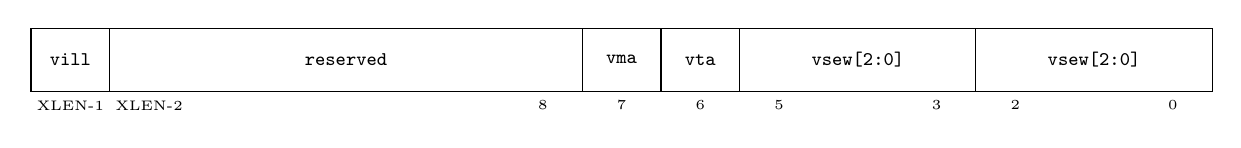
\begin{tikzpicture}
	\def\bitheight{0.4}

	\draw (0,0) rectangle (1, 2 * \bitheight);
	\node at (0.5, \bitheight) {\scriptsize \texttt{vill}};
	\node[below] at (0.5, 0) {\tiny XLEN-1};

	\draw (1,0) rectangle (7, 2 * \bitheight);
	\node at (4, \bitheight) {\scriptsize \texttt{reserved}};
	\node[below] at (1.5, 0) {\tiny XLEN-2};
	\node[below] at (6.5, 0) {\tiny 8};

	\draw (7,0) rectangle (8, 2 * \bitheight);
	\node at (7.5, \bitheight) {\scriptsize \texttt{vma}};
	\node[below] at (7.5, 0) {\tiny 7};

	\draw (8,0) rectangle (9, 2 * \bitheight);
	\node at (8.5, \bitheight) {\scriptsize \texttt{vta}};
	\node[below] at (8.5, 0) {\tiny 6};

	\draw (9,0) rectangle (12, 2 * \bitheight);
	\node at (10.5, \bitheight) {\scriptsize \texttt{vsew[2:0]}};
	\node[below] at (9.5, 0) {\tiny 5};
	\node[below] at (11.5, 0) {\tiny 3};

	\draw (12,0) rectangle (15, 2 * \bitheight);
	\node at (13.5, \bitheight) {\scriptsize \texttt{vsew[2:0]}};
	\node[below] at (12.5, 0) {\tiny 2};
	\node[below] at (14.5, 0) {\tiny 0};
\end{tikzpicture}
\caption{Поля регистра vtype}
\label{fig:vtype}
\end{figure}

\begin{itemize}
	\item \texttt{vill} -- флаг, указывающий на нелегальное значение
	\item \texttt{vma} -- если 0, то немаскированные элементы сохраняют свои значения
	после операций, если 1, то они могут как сохранить, так и быть переписаны единицами
	\item \texttt{vta} -- аналогично \texttt{vma}, только для элементов, которые
	находятся за текущей длиной вектора
	\item \texttt{vsew} -- текущее значение размера одного элемента (Selected Element
	Width, SEW)

	\begin{table}[h]
	\centering
	\begin{tabular}{|c|c|c|c|}
		\hline
		\multicolumn{3}{|c|}{vsew[2:0]} & SEW \\
		\hline
		0 & 0 & 0 & 8 \\
		\hline
		0 & 0 & 1 & 16 \\
		\hline
		0 & 1 & 0 & 32 \\
		\hline
		0 & 1 & 1 & 64 \\
		\hline
		1 & X & X & Reserved \\
		\hline
	\end{tabular}
	\caption{Соответствие между vsew[2:0] и SEW}
	\label{tab:vsew}
	\end{table}

	Значение SEW -- это размер в битах одного скалярного значения внутри векторного
	регистра.
	Соответственно, количество элементов в одном векторном регистре вычисляется как
	$\text{VLEN} / \text{SEW}$. В таблице~\ref{tab:sew} приведен пример для VLEN~=~128 бит.

	\begin{table}[H]
	\centering
	\begin{tabular}{|c|c|}
		\hline
		\texttt{SEW} & Количество элементов \\
		\hline
		8 & 16 \\
		\hline
		16 & 8 \\
		\hline
		32 & 4 \\
		\hline
		64 & 2 \\
		\hline
	\end{tabular}
	\caption{Пример для VLEN = 128 бит}
	\label{tab:sew}
	\end{table}

	\item \texttt{vlmul} -- текущее значение размера группы векторных регистров (Length
	Multiplier, LMUL)
\end{itemize}

Векторные регистры могут быть сгруппированы, чтобы одна векторная инструкция могла
оперировать сразу с несколькими векторными регистрами. Это повышает эффективность
обработки данных, позволяя работать сразу с несколькими регистрами (т.~е. с векторами
увеличенной длины). Значение LMUL представляет собой количество векторных регистров,
сгруппированных вместе.

Кроме того, LMUL может быть дробным значением. Дробное LMUL означает, что используется
только часть бит векторного регистра.

Таким образом, мы можем вычислить максимальное количество скалярных элементов, которыми
может оперировать одна векторная инструкция с текущими SEW и LMUL, как $\text{VLMAX} =
\text{LMUL} * \text{VLEN} / \text{SEW}$.

\item Регистр \texttt{vl} является read-only CSR и может быть обновлен только с помощью
специальных инструкций \texttt{vset\{i\}vl\{i\}}.

Данный регистр хранит в себе беззнаковое целочисленное значение, определяющее, с
каким количеством скалярных элементов будет взаимодействовать векторная инструкция.

\item Регистр \texttt{vlenb} является read-only CSR, который хранит в себе длину одного
векторного регистра в байтах, т.~е. $\text{VLEN} / 8$.

\end{itemize}

\subsection {Соглашение о вызовах}
\label{riscv:callconv}

Соглашение о вызовах (Calling Convention) -- набор правил, являющихся часть ABI (Application
Binary Interface), и определяющих особенности вызова функций. Этими правилами определяются
способы передачи аргументов функции и получения результата ее работы (через регистры процессора 
и/или через стек, порядок размещения аргументов), а также способы вызова и возврата из функций.
Далее в этом разделе я рассмотрю соглашение о вызовах для функций с векторными аргументами и
возвращаемыми значениями.

Для передачи векторных аргументов в функции существует несколько правил. Одно из таких правил
говорит, какие регистры должны использоваться для передачи аргументов и возвращаемого значения,
а какие регистры (точнее, их значения) должны быть сохранены между вызовами.
Регистр \texttt{v0} используется для передачи аргументов с типом векторной маски (т.~е. различные 
типы \texttt{vbool}) и для возвращаемого значения соответствующего типа. Регистры \texttt{v8}-\texttt{v23}
используются для передачи обычных векторных аргументов, кортежных векторных типов и оставшихся
аргументов с типом векторной маски. Эти же регистры используются для возвращаемого функцией
значения с одним из вышеуказанных типов.

Также, должно быть обеспечено сохранение значений регистров \texttt{v1}-\texttt{v7} и
\texttt{v24}-\texttt{v31}.

И последнее в списке, но не по важности, правило, по которому выбираются векторные регистры для
расположения на них аргументов. В первую очередь, мы должны выбрать некоторый последовательный
набор регистров, на котором может поместиться данный аргумент. Например, для типа \texttt{vint64m2\_t}
это может быть \texttt{v8}-\texttt{v9}, но не может быть \texttt{v8} и \texttt{v10}. Второй пункт
в данном правиле говорит о том, что номер первого регистра в данном наборе должен быть кратен значению
LMUL. Например, для типа \texttt{vint64m4\_t} это могут быть наборы \texttt{v8}-\texttt{v11} или
\texttt{v12}-\texttt{v15}, но не \texttt{v9}-\texttt{v12}.

Следует подчеркнуть, что поиск подходящего набора регистров каждый раз начинается с \texttt{v8},
следовательно, существует возможность, что номер первого векторного регистра из набора,
присвоенного векторному аргументу может быть меньше номера первого векторного регистра из набора,
присвоенного одному из предыдущих векторных аргументов. Например, для некоторой функции \texttt{void
foo (vint64m1\_t a, vint64m4\_t b, vint64m2\_t c)}, аргумент \texttt{a} будет располагаться на 
регистре \texttt{v8}, аргумент \texttt{b} на регистрах \texttt{v12}-\texttt{15}, а аргумент \texttt{c}
на регистрах \texttt{v10}-\texttt{v11}. 

\newpage
